\documentclass[tikz,border=5pt]{standalone}
\usetikzlibrary{calc,positioning,intersections,shadows.blur,decorations.pathmorphing,patterns,shapes.callouts}

\definecolor{moonGray}{RGB}{180,180,180}
\definecolor{craterGray}{RGB}{120,120,120}
\definecolor{spaceBlue}{RGB}{10,10,40}
\definecolor{sunlight}{RGB}{255, 215, 0}
\definecolor{sunOrange}{RGB}{255, 165, 0}
\definecolor{earthBlue}{RGB}{60,170,255}
\definecolor{earthGreen}{RGB}{40,140,60}

\begin{document}
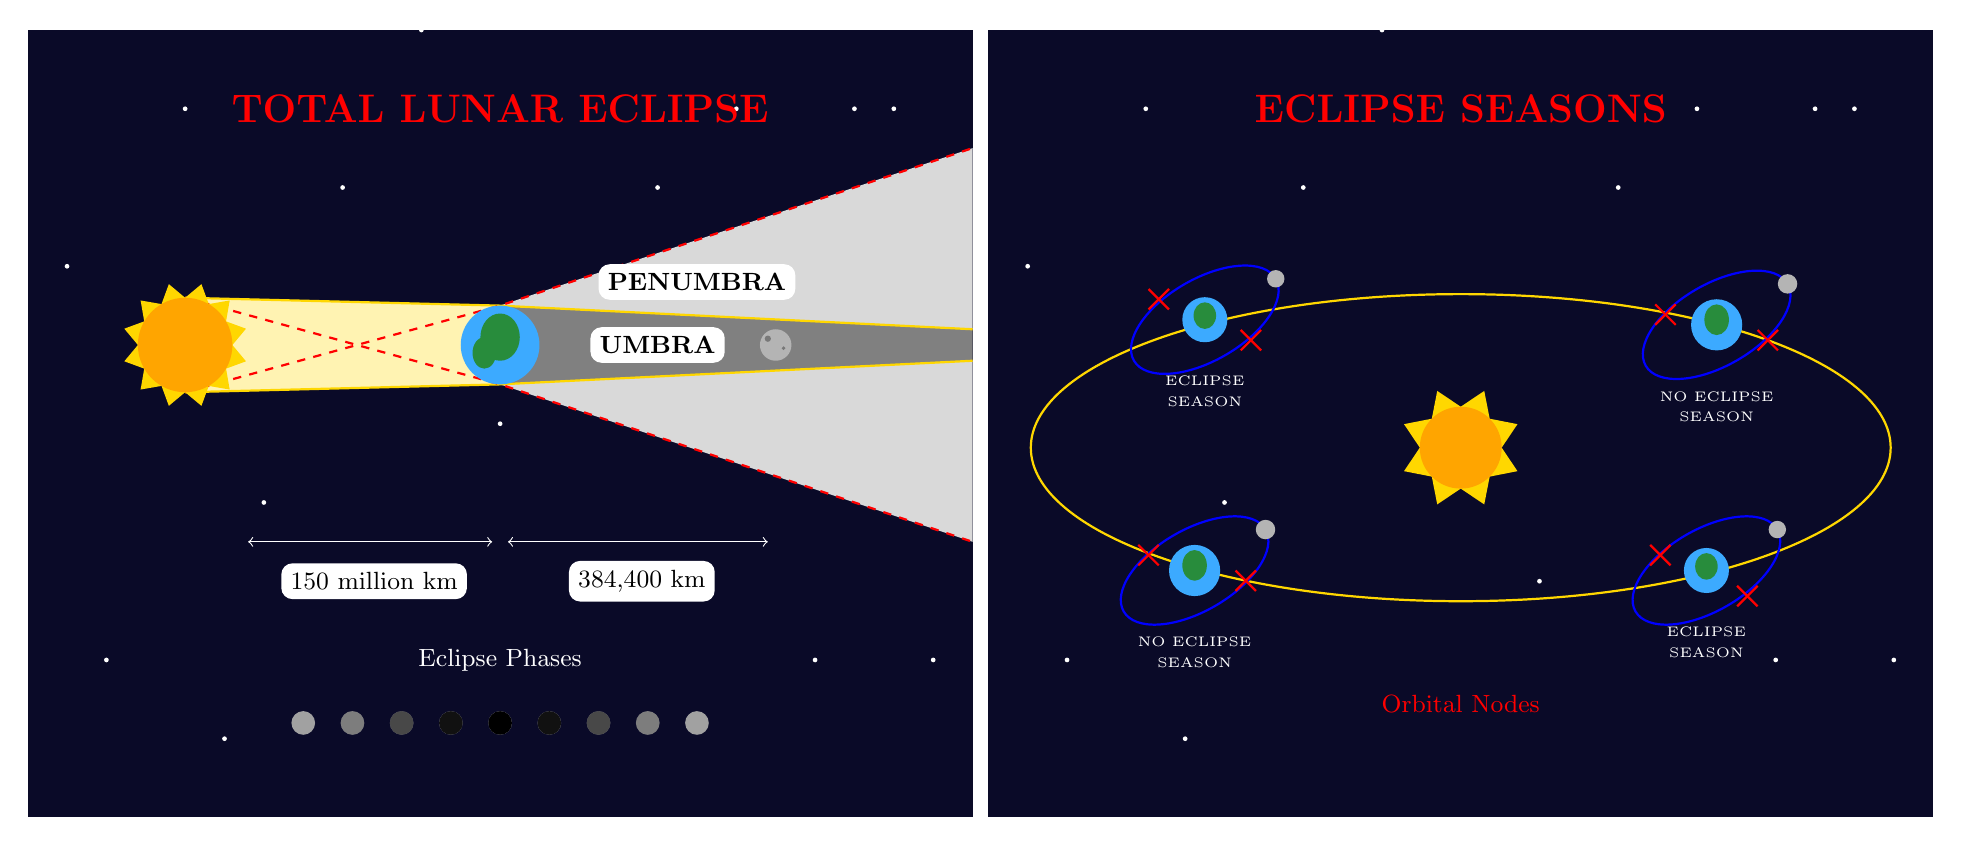
\begin{tikzpicture}[scale=1]

% Left diagram - Total Lunar Eclipse (more compact and square)
\begin{scope}[shift={(-6,0)}]
% Space background (square)
\fill[spaceBlue] (-6,-6) rectangle (6,4);

% Add stars
\foreach \x/\y in {-5/-4, -4/3, -3/-2, -1/4, 1/-3, 3/3, 4/-4, 5/3, -5.5/1, -3.5/-5, -2/2, 0/-1, 2/2, 4.5/3, 5.5/-4}
{
    \fill[white] (\x,\y) circle (0.03);
}

% Title
\node[red, font=\Large\bfseries] at (0,3) {TOTAL LUNAR ECLIPSE};

% Before Earth: Yellow light region between yellow rays
\fill[sunlight!30] (-4,0.6) -- (0,0.5) -- (0,-0.5) -- (-4,-0.6) -- cycle;

% After Earth: Penumbra regions (lighter gray) - extended to right edge
\fill[gray!30] (0,0.5) -- (6,0.2) -- (6,2.5) -- (0,0.5) -- cycle;  % Upper penumbra
\fill[gray!30] (0,-0.5) -- (6,-0.2) -- (6,-2.5) -- (0,-0.5) -- cycle; % Lower penumbra

% After Earth: Umbra region (darker gray) - extended to right edge
\fill[gray] (0,0.5) -- (6,0.2) -- (6,-0.2) -- (0,-0.5) -- cycle;

% Yellow light rays from sun (non-crossing, extended to right edge)
\draw[sunlight, thick] (-4,0.6) -- (0,0.5) -- (6,0.2);  % North pole of sun to north pole of earth, extended
\draw[sunlight, thick] (-4,-0.6) -- (0,-0.5) -- (6,-0.2); % South pole of sun to south pole of earth, extended

% Red penumbra boundaries (dashed, crossing rays) - extended to right edge
\draw[red, dashed, thick] (-4,0.6) -- (0,-0.5) -- (6,-2.5); % North pole of sun to south pole of earth, extending
\draw[red, dashed, thick] (-4,-0.6) -- (0,0.5) -- (6,2.5);  % South pole of sun to north pole of earth, extending

% Sun with triangular flame corona (moved closer)
\begin{scope}[shift={(-4,0)}]
    % Triangular flames around the sun
    \foreach \angle in {0,30,60,90,120,150,180,210,240,270,300,330}
    {
        \fill[sunlight] (0,0) -- (\angle:0.6) -- (\angle+15:0.8) -- (\angle+30:0.6) -- cycle;
    }
    
    % Inner sun core
    \fill[sunOrange] (0,0) circle (0.6);
\end{scope}

% Earth (same size)
\fill[earthBlue] (0,0) circle (0.5);
\fill[earthGreen] (0,0.1) ellipse (0.25 and 0.3);
\fill[earthGreen] (-0.2,-0.1) ellipse (0.15 and 0.2);

% Moon (moved closer)
\fill[moonGray] (3.5,0) circle (0.2);
% Moon craters
\fill[craterGray] (3.4,0.08) circle (0.04);
\fill[craterGray] (3.6,-0.04) circle (0.025);

% Labels
\node[black, fill=white, font=\small\bfseries, rounded corners] at (2.5,0.8) {PENUMBRA};
\node[black, fill=white, font=\small\bfseries, rounded corners] at (2.0,0.0) {UMBRA};

% Distance measurements (adjusted)
\draw[<->, white] (-3.2,-2.5) -- (-0.1,-2.5);
\node[black, fill=white, font=\small, rounded corners] at (-1.6,-3.0) {150 million km};

\draw[<->, white] (0.1,-2.5) -- (3.4,-2.5);
\node[black, fill=white, font=\small, rounded corners] at (1.8,-3) {384,400 km};

% Eclipse phases at bottom
\node[font=\small, white] at (0,-4) {Eclipse Phases};
\foreach \x/\opacity in {-2.5/0.1, -1.875/0.3, -1.25/0.6, -0.625/0.9, 0/1, 0.625/0.9, 1.25/0.6, 1.875/0.3, 2.5/0.1}
{
    \fill[moonGray] (\x,-4.8) circle (0.15);
    \fill[black, opacity=\opacity] (\x,-4.8) circle (0.15);
}
\end{scope}

% Right diagram - Eclipse Seasons (tilted perspective from left side)
\begin{scope}[shift={(6.2,0)}]
% Space background
\fill[spaceBlue] (-6,-6) rectangle (6,4);

% Add stars
\foreach \x/\y in {-5/-4, -4/3, -3/-2, -1/4, 1/-3, 3/3, 4/-4, 5/3, -5.5/1, -3.5/-5, -2/2, 0/-1, 2/2, 4.5/3, 5.5/-4}
{
    \fill[white] (\x,\y) circle (0.03);
}

% Title
\node[red, font=\Large\bfseries] at (0,3) {ECLIPSE SEASONS};

\begin{scope}[scale=1.3, yshift=-20.0]

% Sun at center
\begin{scope}[shift={(0,-0.3)}]
    \foreach \angle in {0,45,90,135,180,225,270,315}
    {
        \fill[sunlight] (0,0) -- (\angle:0.4) -- (\angle+22.5:0.6) -- (\angle+45:0.4) -- cycle;
    }
    \fill[sunOrange] (0,0) circle (0.4);
\end{scope}

% Earth's orbit (ecliptic plane) - shown as tilted ellipse from left perspective
\draw[sunlight, thick] (0,-0.3) ellipse (4.2 and 1.5);

% Four Earth-Moon system positions aligned with line of nodes
% Position 1: Eclipse season - upper right along line of nodes
\begin{scope}[shift={(2.5,0.9)}]
    % Earth
    \fill[earthBlue] (0,0) circle (0.25);
    \fill[earthGreen] (0,0.05) ellipse (0.12 and 0.15);
    
    % Moon's orbit - flattened, tilted 15 degrees to the right
    \draw[blue, thick, rotate=30] (0,0) ellipse (0.8 and 0.4);
    
    % Moon at position (moved to top-left on orbit, larger)
   \fill[moonGray] ({0.8*cos(30)},{0.8*sin(30)}) circle (0.095);
    
    \node[white, font=\tiny, rounded corners] at (0,-0.7) {NO ECLIPSE};
    \node[white, font=\tiny, rounded corners] at (0,-0.9) {SEASON};
\end{scope}

% Position 2: No eclipse season - perpendicular to line of nodes (left side)
\begin{scope}[shift={(-2.5,0.95)}]
    % Earth
    \fill[earthBlue] (0,0) circle (0.22);
    \fill[earthGreen] (0,0.04) ellipse (0.11 and 0.13);
    
    % Moon's orbit - flattened, tilted 15 degrees to the right
    \draw[blue, thick, rotate=30] (0,0) ellipse (0.8 and 0.4);
    
    % Moon at position (moved to top-left on orbit, larger)
   \fill[moonGray] ({0.8*cos(30)},{0.8*sin(30)}) circle (0.085);
    
    \node[white, font=\tiny, rounded corners] at (0.0,-0.6) {ECLIPSE};
    \node[white, font=\tiny, rounded corners] at (0.0,-0.8) {SEASON};
\end{scope}

% Position 3: Eclipse season - lower left along line of nodes
\begin{scope}[shift={(-2.6,-1.5)}]
    % Earth
    \fill[earthBlue] (0,0) circle (0.25);
    \fill[earthGreen] (0,0.05) ellipse (0.12 and 0.15);
    
    % Moon's orbit - flattened, tilted 15 degrees to the right
    \draw[blue, thick, rotate=30] (0,0) ellipse (0.8 and 0.4);
    
    % Moon at position (moved to top-left on orbit, larger)
   \fill[moonGray] ({0.8*cos(30)},{0.8*sin(30)}) circle (0.095);
    
    \node[white, font=\tiny, rounded corners] at (0,-0.7) {NO ECLIPSE};
    \node[white, font=\tiny, rounded corners] at (0,-0.9) {SEASON};
\end{scope}

% Position 4: No eclipse season - perpendicular to line of nodes (right side)
\begin{scope}[shift={(2.4,-1.5)}]
    % Earth
    \fill[earthBlue] (0,0) circle (0.22);
    \fill[earthGreen] (0,0.04) ellipse (0.11 and 0.13);
    
    % Moon's orbit - flattened, tilted 15 degrees to the right
    \draw[blue, thick, rotate=30] (0,0) ellipse (0.8 and 0.4);
    
    % Moon at position (moved to top-left on orbit, larger)
   \fill[moonGray] ({0.8*cos(30)},{0.8*sin(30)}) circle (0.085);
    
    \node[white, font=\tiny, rounded corners] at (0.0,-0.6) {ECLIPSE};
    \node[white, font=\tiny, rounded corners] at (0.0,-0.8) {SEASON};
\end{scope}

% Line of nodes indication
\node[red, font=\small, rounded corners] at (0.0,-2.8) {Orbital Nodes};

% Add red crosses at 4 random locations using for loop
\foreach \x/\y in {-2.1/-1.6, -3.05/-1.35, -2.05/+0.75, -2.95/+1.15, +3.0/+0.75, +2.0/+1.0, +1.95/-1.35, +2.8/-1.75} {
    \draw[red, thick] (\x-0.1,\y-0.1) -- (\x+0.1,\y+0.1);
    \draw[red, thick] (\x-0.1,\y+0.1) -- (\x+0.1,\y-0.1);
}

\end{scope}

\end{scope}

\end{tikzpicture}
\end{document}